\documentclass[thesis]{cluu}

\usepackage[style=cluu]{biblatex}
\usepackage{tabularx}
\usepackage[acronym]{glossaries}
\usepackage{tikz}
\usetikzlibrary{arrows.meta,positioning,shapes.geometric,fit}
\usepackage{cleveref}
\usepackage{graphicx}
\graphicspath{ {./images/} }
\usepackage{adjustbox}

\makeglossaries

\newacronym{ai}{AI}{Artificial Intelligence}
\newacronym{ml}{ML}{Machine Learning}
\newacronym{nlp}{NLP}{Natural Language Processing}
\newacronym{call}{CALL}{Computer-Assisted Language Learning}
\newacronym{icall}{icall}{Intelligent CALL}
\newacronym{capt}{CAPT}{Computer-Assisted Pronunciation Training}
\newacronym{json}{JSON}{JavaScript Object Notation}
\newacronym{llm}{LLM}{Large Language Model}
\newacronym{nlg}{NLG}{Natural Language Generation}
\newacronym{md}{MD}{Mispronunciation Detection}
\newacronym{mdd}{MDD}{Mispronunciation Detection and Diagnosis}
\newacronym{ctc}{CTC}{Connectionist Temporal Classification}
\newacronym{cnn}{CNN}{Convolutional Neural Network}
\newacronym{sota}{SotA}{State-of-the-Art}
\newacronym{fleurs}{FLEURS}{Few-shot Learning Evaluation of Universal Representations of Speech}
\newacronym{l2}{L2}{second language}
\newacronym{l1}{L1}{first language}
\newacronym{sla}{SLA}{second-language acquisition}
\newacronym{nn}{NN}{neural network}
\newacronym{tts}{TTS}{Text-to-Speech}
\newacronym{asr}{ASR}{automatic speech recognition}
\newacronym{ipa}{IPA}{the International Phonetic Alphabet}
\newacronym{g2p}{G2P}{Grapheme-to-Phoneme}
\newacronym{wals}{WALS}{the World Atlas of Linguistic Structure}
\newacronym{mfa}{MFA}{Montreal Forced Aligner}

% Define tikz styles to reuse in figures
\usepackage[edges]{forest}
\usetikzlibrary{arrows.meta} % for Latex arrowheads

\forestset{
  box/.style={
    draw, rounded corners=2mm, thick,
    minimum height=9mm, align=center
  },
  internal/.style={box, fill=blue!10},
  posleaf/.style={box, fill=green!15},
  negleaf/.style={box, fill=red!15},
  edgelabel/.style={midway, sloped, above},
}

% Define a new counter for paragraphs (delete when paper is done)
\newcounter{paranum}
% Command to increment and display the paragraph number for initial planning
\newcommand{\numberedparagraph}{\par\refstepcounter{paranum}\textbf{[\theparanum] }}

\newcommand{\todo}[1]{\textcolor{red}{#1}}

% use Doulos SIL for IPA transcriptions
\newfontfamily\ipafont{Doulos SIL}[Scale=MatchLowercase]
\newcommand{\ipa}[1]{{\ipafont #1}}

%ThesisProject is auto updated by zotero
\addbibresource{ThesisProject.bib}

\begin{document}
\title{My thesis}
\author{Peter Cady}
% \date{...}
\supervisors{Johan Sjons, Uppsala University\\
  Jim O' Regan, KTH Royal Institution of Technology}
% Use \supervisor (without s at end) if you have only one

\maketitle

\begin{abstract}
    \numberedparagraph summarize the motivation
    \numberedparagraph problem overview
    \numberedparagraph experiment
    \numberedparagraph main findings and contributions.
\end{abstract}

\tableofcontents

\addchap{Preface}
% with \addchap instead of \chapter it isn't numbered.
\addchap{Acknowledgements}
Thank my partner
Thank Johan
I would especially like to thank Jim O' Regan for all his thought-provoking insights, encouragement, and advice, which were crucial for me getting my bearings in a project which pushed me to grow beyond my limits. The process was deeply meaningful to me. Thank you.
Thank Greg and Conchúr
Thank examiner

\printglossary[type=\acronymtype]

\printglossary

\chapter{Introduction}
\numberedparagraph Lead work here. Outline modern context of minority languages in nlp. Introduce Irish context in this framework.
\todo{revisit introduction, try to lead with an impactful framing of the motivation of the work.}
Language competency is crucial in securing opportunities in the workplace as well as for accessing services and exercising rights in society at large. Language technologies have become central to many of the ways we interact with each other and society, for both good and ill. Such technologies are often identified as promising tools to promote language learning, but are also implicated in the coalescence of online interaction around a few dominant languages such as English. Low-resource languages struggle to keep pace with the most recent technological advancements given the relative scarcity of data they are faced with, necessitating 

\numberedparagraph Reiterate need for a solution, lead into research question explanation
These 

\numberedparagraph Outline key goals of thesis
In this thesis we explore the feasibility of two primary methods of overcoming the scarcity of phonetically annotated \gls{l2} Irish learner data for \gls{md} applications. One approaches the problem with ensembles of monolingual \gls{asr} models for which data scarcity less acute, and another using a schema of data generation by leveraging established \gls{tts} systems to approximate learner speech: a potential low-cost alternative to large-scale phonetic annotation. By exploring these approaches, we aim to illuminate possible ways forward for low-resource language communities interested in developing automated technologies for language learning and pronunciation training.

\numberedparagraph CAPT intro
\textcite{chenComputerassistedPronunciationTraining2016} CAPT review, emphasis on teaching and learning, prosody

\numberedparagraph ASR intro

\chapter{Background \& Related works}
\numberedparagraph Short overview of background section

In the following section we will outline the context motivating our current work with relation to \gls{nlp} research for minority languages. We begin by exploring the different themes at play in the current work, summarizing the lay of the land, before digging into the ongoing research in these areas to rectify some thusfar recalcitrant problems hindering more equal access to the benefits of our time's rapid advances in language technology. 

\section{Irish \& The Predicament of Minority Languages}

\numberedparagraph introduce need for general-use systems.
Developing language technologies that can scale beyond the language they are designed for is no new goal for \gls{nlp} research. The value of such a property is apparent: transferring an existing system seamlessly to another language could potentially save significant resources for language communities without the ability to fund such system development themselves. Actually achieving this goal in practice, however, is no simple endeavor, typically requiring some level of linguistic awareness which is all-to-often lamentably absent \parencite{benderAchievingEvaluatingLanguageIndependence2011,joshiStateFateLinguistic2021,hedderichSurveyRecentApproaches2021,inter alia}. For example, success in applying supposedly language independent word-based n-gram approaches to languages rests on its level of inflectional morphology: the lower the better. Higher morphological complexity together with variations in word order raise data sparsity problems which n-gram approaches rooted in English struggle to handle \parencite{benderAchievingEvaluatingLanguageIndependence2011}. This should come as no surprise, given the relatively fixed word order and low levels of inflectional morphology present in English, but it illustrates a need for caution: systems developed for a given language may make implicit assumptions about language structure which do not generalize well. Linguistic typology can provide important clues as to what features are shared between the original development language and possible languages of extension for a system. Information of this kind has, for many of the worlds languages, already been gathered by linguists. Perhaps the most renowned database of typological information is \gls{wals} \parencite{matthewdryerWorldAtlasLanguage2024}, a free, online resource currently boasting 152 chapters with detailed descriptions of 192 linguistic features spanning over 2,600 of the world's languages. How a language is communicated through script is also a point of complication for \gls{nlp} research, with \textcite{manoharWhatLostNormalization2024} implicating standard normalization praxis when comparing ASR models as artificially inflating scores of languages using Indic scripts. Correctly segmenting continuous-script languages like Chinese is another area of ongoing research with clear implications for downstream performance. \todo{get a good reference here and clean up transitions}. By explicitly mobilizing linguistic knowledge already painstakingly gathered by linguistic typologists, we can identify where languages agree, where they differ, and hopefully identify implicit, ungeneralizable assumptions underpinning our approaches earlier in the design stage.

\numberedparagraph language disparity in lang tech. 
Despite the claims of language-agnostic systems often touted by proponents of emerging \gls{ai} technologies, these systems have often fallen well short of such promise. The overwhelming majority of the world's languages have no footprint in emerging language technologies \parencite{joshiStateFateLinguistic2021}. In the past, building \gls{nn}-based language technologies demanded immense quantities of labeled data: a high bar of entry to the language communities of those languages with limited if any access to such resources, and an ongoing issue which continues to stimulate a body of research dedicated to overcoming such issues(see \textcite{magueresseLowresourceLanguagesReview2020} for an overview). For languages where data availability is no obstacle, research and development can proceed unfettered by the prohibitive cost of curating datasets from scratch. As our daily lives grow increasingly integrated with the digital realm, language communities without the same support are obliged to switch to more digitally dominant languages (often English) to gain access to these new resources, narrowing the opportunities to engage with resources and services through the medium of their mother tongue \parencite{nichasaideCanWeDefuse2019}. A particularly sobering taxonomy illustrating the states of languages facing such disparities is formulated by \textcite{joshiStateFateLinguistic2021} and reproduced in \cref{tab:data_availability} on page \pageref{tab:data_availability}, which outlines the states and challenges faced by languages in resource terms in the digital space, and how dominant a small group of languages are within it. Of particular note for the priviledged few that find themselves at the top of the heap is their typological similarity, being drawn as they are from a few dominant language families (and even dominant branches within these larger families). This state of affairs constitutes a sort of typological echo-chamber for the cutting edge of \gls{nlp} developments, a point which we will return to shortly.

\begin{table}[h]
    \centering
    \begin{tabularx}{\textwidth}{|X|p{2cm}|p{1.75cm}|}
        \hline
        \textbf{Class Descriptions} & \textbf{Example Languages} & \textbf{\% of total languages}\\ \hline
        \textbf{0} The Left-Behinds: Virtually ignored in language technology. Exceptionally limited resources available, even with respect to unlabeled data. & Dahalo, Bora & 88.17\%\\ \hline
        \textbf{1} The Scraping-Bys: Some unlabeled data. With organized promotion and data collection, there is hope for improvement in coming years. & Fijian, Navajo & 8.93\%\\ \hline
        \textbf{2} The Hopefuls: Limited labeled data. Support communities help these languages survive, and there is promise for \gls{nlp} tools in the near term. & Zulu, \textbf{Irish} & 0.76\%\\ \hline
        \textbf{3} The Rising Stars: Strong web presence and thriving cultural community online. Lacking in labeled data. Good potential for \gls{nlp} tool development for these languages. & Indonesian, Hebrew & 1.13\%\\ \hline
        \textbf{4} The Underdogs: Much unlabeled data, and less but still significant labeled data. Dedicated investment from NLP communities. & Russian, Dutch & 0.72\%\\ \hline
        \textbf{5} The Winners: Dominant online presence with massive investment and resources. & English, German & 0.28\%\\ \hline
    \end{tabularx}
    \caption{Data availability \& status taxonomy of languages adapted from work by \textcite{joshiStateFateLinguistic2021}.}
    \label{tab:data_availability}
\end{table}
\numberedparagraph set the Irish case in this context, outline challenges currently undertaken by developers

Despite some advantages not afforded other minority languages, Irish still finds itself struggling to maintain a footing in the the digital realm, placed by \textcite{joshiStateFateLinguistic2021} in class 2 of the taxonomy outlined in \cref{tab:data_availability}. It enjoys ongoing investment by the Irish state, nominal status of Irish as the first national language of the Republic of Ireland, and research dedicated to its promotion (e.g. through the ABAIR initiative dedicated to developing speech technologies for Irish, see \parencite{chasaideABAIRInitiativeBringing2017}). At the same time, it is a typological outlier in several respects: it is a verb-initial language with relatively complex inflectional morphology, and a distinct (though still Latin-based) orthography. Features like these put Irish at odds with many languages in the high-resource echo-chamber, complicating the ability to leverage cutting-edge models to linguistic features with no representation in a model's training data. Furthermore, though we have treated Irish as a single entity thus far, an important complication reveals itself in the discontiguous nature of the Irish-speaking areas, referred to as \textit{the Gaeltachtaí}. Each of the three main areas (i.e. Ulster, Connacht, and Munster \ref{fig:gaeltacht}) speaks markedly distinct varieties of Irish, \todo{find a picture for this} necessitating adequate labeled data if these groups are to be adequately serviced by new technologies. In the face of such limitations, today's data-hungry tools simply cannot be expected to perform to the same level on languages like Irish without the same access to resources. It should be noted that the pretraining/finetuning paradigm of recent massive multilingual models does mitigate this demand for data somewhat by leveraging unlabeled cross-lingual data, reducing the need for labeled data in the language finetuned to \parencite{hedderichSurveyRecentApproaches2021,ranathungaNeuralMachineTranslation2021,joshiStateFateLinguistic2021}, but for other languages without even minimal labeled data to their name, this is a small comfort.\todo{which survey references do I want to use?}

\todo{placeholder. find good open source gaeltacht image}
\begin{figure}[h]
    \caption{Area of the Gaeltachtaí (Irish-speaking areas of Ireland) colored in green}
    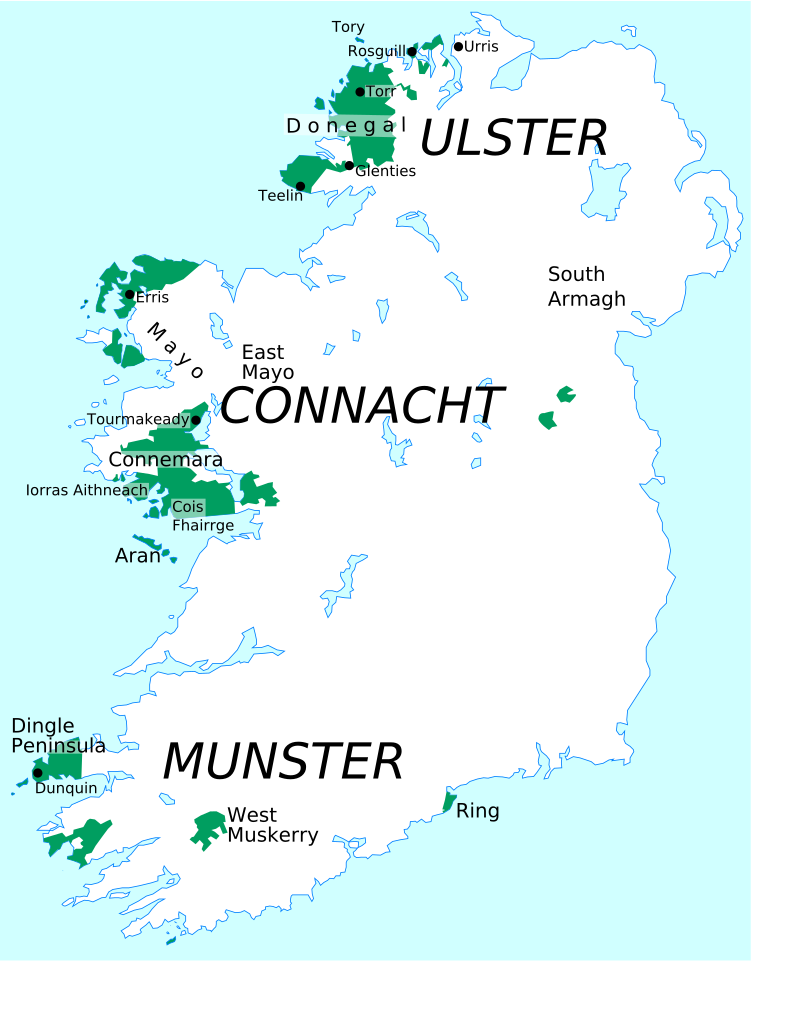
\includegraphics[width=8cm]{Gaeltachtai_le_hainmneacha2.png}
    \centering
    \label{fig:gaeltacht}
    \caption{The original uploader was Angr at English Wikipedia. - Transferred from en.wikipedia to Commons., CC BY-SA 3.0, https://commons.wikimedia.org/w/index.php?curid=3532749}
\end{figure} 

\numberedparagraph problems to be solved for Irish speakers 
Though the hurdles facing the Irish language in the digital sphere are a relatively recent concern, the issues facing it in the real world are anything but. It is currently classified by UNESCO as being \textit{definitely endangered} \parencite{moseleyAtlasWorldsLanguages2010}, following centuries of varying rates of contraction due to encroachment by English \todo{give some more explanation of the history, handle with care}. Irish survives as a community languages in the aforementioned Gaeltacht areas, though even there it is estimated that only 24\% of inhabitants speak Irish on a daily basis \parencite{nichasaideSPEECHTECHNOLOGYDOCUMENTATION}. Despite this worrying state of Irish as a \gls{l1}, it is comparatively strong as a \gls{l2} \todo{dig up ref from broin about second language stats}. A growing number of parents seek Irish-medium education for their children outside the Gaeltacht, and immersive summer courses remain popolar among adults looking to learn or reconnect with the language. This encouraging \gls{l2} engagement intersects with thorny issues of supply, however, as many of the teachers are not themselves native speakers with an accompanying native grasp of the structure and sound of the language \parencite{nichasaideSPEECHTECHNOLOGYDOCUMENTATION,nichasaideCanWeDefuse2019}. This limited native speaker model for \gls{l2} speakers is particularly problematic for teaching pronunciation, complicating the acquisition of some sound contrasts critical to disambiguating the Irish grammar. Perhaps chiefly among these, contrasts between the secondary articulation of consonants into \textit{palatalised} and \textit{velarised} variants play an instrumental role in a number of grammatical functions, such as in the formation of certain plurals and genitive marking \parencite{snesarevaPalatalizationDublinIrish2016,gabrieleEnglishInfluenceL2,broinNewUrbanIrish,stensonModernIrishComprehensive2020}. Since the Roman alphabet doesn't provide symbols for this distinction, Irish orthography marks it via adjacent letters as seen in \todo{give sub-table references} of \cref{tab:sound_contrasts}: so-called \textit{slender} vowels ('i' and 'e') flanking a consonant denote \textit{palatalisation}, while \textit{broad} vowels ('a', 'o', and 'u') mark \textit{velarisation} \parencite{stensonModernIrishComprehensive2020}. Mutation effects are another pervasive element of the Irish grammar relying on sound alterations, the most common of which are \textit{lenition} and \textit{eclipsis}. \textit{Lenition},traditionally termed \textit{séimhiú} (/\ipa{ˈʃeːvʲuː}/), is commonly marked with an 'h' following the lenited consonant as seen on \cref{tab:sound_contrasts}, and originally denoted a weakening in the manner of articulation, though the relationship between consonants and their lenited versions is less immediately apparent now for some consonants \parencite{stensonModernIrishComprehensive2020}. \textit{Eclipsis}, traditionally \textit{úru} (/\ipa{ˈʊɾˠuː}/), involves replacing the original consonant with a nasalized or voiced version, and is denoted by appending the new sound character before the consonant being eclipsed\ref{tab:sound_contrasts} \todo{add sub-table refs and double check if this description covers all the bases}. These and other structural underpinnings of the language can have far-reaching implications for intelligability if not adequately mastered by students. Indeed, a study undertaken by\textcite{broinNewUrbanIrish} reveals that realisations of phonological like those above are over 50\% on average for urban speakers, with some as high as 82\%---a stark departure from their gaeltacht counterparts which lie below 10\%. Providing wider access to better native models of pronunciation --- not to mention native models of morphology --- could do much to close this gap, making mutual intelligability more attainable between gaeltacht and urban speakers. 

\begin{table}[ht]
  \centering
  \caption{Examples use of mutation effects (séimhiú \& úru) as well as consonant velarisation \& palatalisation}
  \begin{tabular}{l r}
    Phoneme & Count \\
    \hline
    /a/ & 42 \\
    /i/ & 35 \\
  \end{tabular}
  \label{tab:sound_contrasts}
\end{table}

\textcite{gabrieleEnglishInfluenceL2} english influence on palatalization and velarization
\textcite{snesarevaPalatalizationDublinIrish2016} how does english influence Irish spoken by dublin bilinguals?
\textcite{broinNewUrbanIrish} differences of irish between cities and gaeltacht
\textcite{nichasaideSPEECHTECHNOLOGYDOCUMENTATION} documentation of Irish with speech tech
\textcite{hedderichSurveyRecentApproaches2021} survey of low resource NLP methods
\textcite{magueresseLowresourceLanguagesReview2020} survey of low resource methods in \gls{nlp}
\textcite{wuTransformerBasedEndtoEnd2021} motivation for phone-based recognition for MDD instead of scoring pronunciations (like GOP)

\section{Second Language Acquisition}

\section{\gls{call} \& \gls{capt}}
The rise of digital technologies is often implicated in the acceleration of already precpitous rates of decline for endangered languages. However, it is a trend that cuts both ways, as the same technologies that squeeze certain languages out of the digital realm are also making space for communities of language learners to come together towards their common goal. The increased presense of technology both in and outside the classroom brings with it broad implications for traditional pedgagogy, enabling more autonomous and flexible modes of learning for students. For language pedgagogy specifically, this has increased the financial viability of courses for endagered or otherwise less commonly taught languages, allowing teachers to draw from a more geographically dispersed enrollment pool and provide courses otherwise impossible to offer /parencite{spolskyHandbookEducationalLinguistics2008}\todo{alter bib entry to reflect book chapter, not whole book}. Furthermore, as prominent \gls{call} software for self-study such as Duolingo, Babbel, and Rosetta Stone proliferate, the advantages of immediate and personalised feeback are increasingly hard to ignore. This new reality has not come without growing pains. Integrating the new digital dimension of the modern language landscape with traditional educational goals has been been an area of longstanding misalignment, limiting fuller realization of their potential \parencite{bajorek2017l2}. Despite these shortcomings, the digial nature of \gls{call} systems has some alluring implications for the viability of individualized pronunciation training.

Effective pronunciation training requires one-on-one interaction between students and teachers. This individualized dynamic generally carries a steep price tag for the student, but \gls{capt} systems can potentially lower this barrier of entry considerably by automating the same kind of undivided feedback in a form scalable to many geographically disperesed students at once.
\textcite{kyriakopoulosDeepLearningApproach2018} capt with phone distances
\textcite{levisCOMPUTERTECHNOLOGYTEACHING2007} overview of technology in pronunciation research (good choice of overview)
\textcite{rogerson-revellComputerAssistedPronunciationTraining2021} survey essay on current status of CAPT circa 2021
\textcite{witt2014computer} scores on a phonemic level GOP. likelihood ratio between forced alignment and max likelihood mohophone loop? aspects of pronunciation teaching overview.

\numberedparagraph aspects of pronunciation
\textcite{wittPhonelevelPronunciationScoring2000} components of pronunciation page 10
\textcite{engstrandFonetikensGrunder2004} check section on prosody for segmental suprasegmental breakdown.
\textcite{mihalicekLanguageFilesMaterials2012} intro to linguistics. maybe good segmental breakdown, havn't found it yet.

\numberedparagraph motivation for language feedback
\textcite{hansenedwardsPhonologySecondLanguage2008} part of a larger work about phonology in 2nd language acquisition (is right reference?)
\textcite{hardisonSecondlanguageSpokenWord2005} effect of perceptual training and phonetic environment. visual cues serve priming role in audiovisual speech processing
\textcite{homaRoleFeedbackCategory} motivation on value of feedback
\textcite{islamExploringSpeechRepresentations2023} example feedback instead of expert feedback.
\textcite{levisTeachingIntonationDiscourse2004} intonation feedback with speech visualization.
\textcite{liPhonemeLevelArticulatorDynamics2011} discussion about phoneme-level speech visualization as tool for feedback
\textcite{lysterOralCorrectiveFeedback2013} Oral corrective feedback in L2 classroom
\textcite{hosseini-kivananiExperimentsASRbasedMispronunciation2021} motivation for non-native error language model

\numberedparagraph short framing of \gls{l2} learner motivation and Language learning
%\hyperlink{sla}{https://en.wikipedia.org/wiki/Theories_of_second-language_acquisition}
\textcite{vanpatten2007theories} second language acquisition
\textcite{bodnarEvaluatingMotivationalImpact2016} motivational impact of call systems
\textcite{mac2023learning} l2 motivation in lMOOCS
\textcite{maclochlainnClickingConnectingL22021} more on lmoocs and participation motivation
\textcite{schmidtChapter2Attention2012} Noticing hypothesis for L2 pedagogy

\numberedparagraph outline CALL and pronunciation training's place within it.
\textcite{eskenaziOverviewSpokenLanguage2009} overview of language tech in education
\textcite{levisCOMPUTERTECHNOLOGYTEACHING2007} pronunciation feedback, appropriateness, goals, and ability for ASR to provide this.
\textcite{volodina2016proceedings} workshop on NLP for CALL and NLP for Language acquisition. good motivation for
\textcite{arnbjornsdottirIntelligentCALLGranular2022} CALL for language learning
\textcite{amrateComputerassistedPronunciationTraining2025} capt overview
\textcite{collinsGaeltechVRMeasuringImpact2019} icall VR application measuring impact of virtual reality.
\textcite{collinsSituatedImmersiveGaming2021} situated learning for Irish. motivation benefits and anxiety reduction
\textcite{kheirAutomaticPronunciationAssessment2023} review of pronunciation assessment

\numberedparagraph how to measure L2 pron proficiency
\textcite{saitoEffectsSecondLanguage2019} framework for conceptualizing measure of instructed L2 pronunciation prof
\textcite{strikComparingDifferentApproaches2009} Differences between error detection and pronunciation scoring
\textcite{wittPhonelevelPronunciationScoring2000} GOP, likelihood of a phone given the acoustic segment. notes highly subjective nature of pronunciation assessment
\textcite{wittAutomaticErrorDetection} auto error detection, where we are and where we need to go. overview of research use in commercial learning software. touches on cross-disciplinary nature of automatic pronunciation training.
\textcite{witt2000use} GOP dissertation
\textcite{sudhakaraImprovedGoodnessPronunciation2019} improved GOP
\textcite{thomsonEffectivenessL2Pronunciation2014} l2 pronunciation effectiveness

\numberedparagraph What are the sources of mispronunciation? What level do they operate at?
\textcite{chenEndtoEndNeuralNetwork2018} speech scoring with e2e systems
\textcite{liMispronunciationDetectionDiagnosis2017} good overview of scoring approaches plus new approach

\numberedparagraph icall in Irish
\textcite{nichiarainDigichaintInteractiveGame2016} icall platform
\textcite{nichiarainScealaiSyntheticVoices2018} icall platform
\textcite{nichiarainUsingSpeechNLP2022} icall for minority languages
\textcite{nichiarainCorpasClisteCreating2022} corpas cliste, data from platforms.

\numberedparagraph Reiterate need for a solution to some of these problems, additionally for learning and teaching to lead into CALL
\textcite{gabrieleEnglishInfluenceL2} english effect on velarization/palatalization
\textcite{holmbergDesigningAddedPedagogical} thesis on designing computer systems for pedagogical value

\numberedparagraph comparison to other CAPT applications (wav2vec2trainer?)
\textcite{ballierUsingWhisperLLM} approach using whisper
\textcite{bannoProficiencyAssessmentL22022} proficiency grading with wav2vec2
\textcite{islamExploringSpeechRepresentations2023} automatic proficiency assessment with exemplar-based approach for 3 levels of proficiency

\numberedparagraph pronunciation trainer with agent interface (which slate talk was this?)
\textcite{bouliannePhonemeTranscriptionEndangered2022} wav2vec2 large for phonetic transciption. good results for little training.

\numberedparagraph Error modeling (systematic vs individual errors: see witt 1999)
\textcite{pisoniHandbookSpeechPerception} particularly phonetic processing and phonological contrast chapters

\numberedparagraph build case for value of corrective feedback in language learning from pedagogical texts
\textcite{bajorek2017l2} language apps are lacking
\textcite{islamExploringSpeechRepresentations2023} example feedback with clustering
\textcite{sheenCorrectiveFeedbackLearner2004} Similarity and difference in corrective feedback and learner uptake (recasts, type of recast important)

\subsection{MDD}
\numberedparagraph Introduce Mispronunciation detection and diagnosis (MDD)
\textcite{fuFullTextDependentEnd2021} data augmentation for MDD
\textcite{kheirMispronunciationDetectionSpeechBlender} MDD with hmm gnn for arabic
\textcite{kheirAutomaticPronunciationAssessment2023} review of MDD capt systems
\textcite{kheirL1awareMultilingualMispronunciation2023} Multilingual MDD framework
\textcite{alrashoudiImprovingMispronunciationDetection2025} MDD for arabic with transofmers
\textcite{kimAutomaticPronunciationAssessment2022} focus more on pron scoring instead of MDD
\textcite{pengStudyFineTuningWav2vec202021} Wav2vec2 for MDD (important)
\textcite{pengTextAwareEndtoendMispronunciation2022} gating strategy (ignore irrelevant parts in transcription) and constrastive loss to reduce objective gap between phoneme recognition and MDD
\textcite{shahinPhonologicalLevelMispronunciationDetection2024} phonological-level MDD (articulatory focus) True acceptance rate, false rejection tc
\textcite{stanleyImprovingL1specificPhonological2012} difference in L1 dependent models vs baseline. how to introduce non native acoustic features. (variant of min phone error training that optimizes on maximizing discriminability between confusable phonetic units in nonnative acoustic space.)
\textcite{xuExploreWav2vec202021} wav2vec2 for MDD

\numberedparagraph describe its relations to ASR
\parencite{barteldsMakingMoreLittle2023} survey of low-resource ASR
\parencite{besacierAutomaticSpeechRecognition2014} survey of low-resource ASR

\chapter{Related Work}
In the following section, we will dive into strategies commonly used to address the problem area outlined above: the place of \gls{asr} in \gls{mdd}, as well as some of the strategies adopted to overcoming the mismatch in objectives between ordinary phoneme recognition and \gls{md}

\section{ASR for MDD}
\textcite{poveyKaldiSpeechRecognition} classic toolkit for asr
\numberedparagraph Outline the function of an asr system.
\textcite{pisoniHandbookSpeechPerception} for perception of sound


\numberedparagraph What types of ASR systems are there? which are we using?
\textcite{hsuHuBERTSelfSupervisedSpeech2021} Hidden unit BERT. provides aligned target labels for model prediction loss

\numberedparagraph Touch on phoneme extraction task and detail fine-tuning procedure
\textcite{agrawalLearningWhenTrust2023} smart weighter mechanism that selects model based on input audio

\numberedparagraph MDD scoring

% forest package for more painless trees
\begin{figure}[t]
\centering
\begin{adjustbox}{max width=\linewidth}
\begin{forest}
for tree={
  edge={-{Latex[length=1.6mm]}},
  l sep=5mm,        % level separation (vertical)
  s sep=2mm          % sibling separation (minimum horizontal)
}
[Transcribed Phonemes, internal
  [Correct Pronunciations, internal
    [True Acceptance, posleaf]
    [False Rejection, negleaf]
  ]
  [Mispronunciations, internal
    [False Acceptance, negleaf]
    [True Rejection, internal
      [Correct Diagnosis, posleaf]
      [Diagnosis Error,  negleaf]
    ]
  ]
]
\end{forest}
\end{adjustbox}
\label{fig:eval}
\caption{Evaluation hierarchy of \gls{md}}
\end{figure}

\section{Ensembling}
\numberedparagraph describe the general strategy of model ensembling
\textcite{fiscus1997post} ROVER ensembling
\textcite{jalalvandAutomaticQualityEstimation2018} novel ROVER approach with quality ranking at segment level

\section{TTS data augmentation}
\textcite{korzekwaComputerassistedPronunciationTraining2022} synthesis approaches to boosting asr
\textcite{shenNaturalTTSSynthesis2018} TTS Tacotron (maybe find google tts paper)

\numberedparagraph connect strategy to current work
\textcite{punjabiLanguageModelBootstrapping2019} bootstrapping data with MT (important)
\textcite{xuIterativePseudoLabelingSpeech2020} multiple iteration of pseudo-labeling on unlabeled data to overcome data scarcity
\textcite{yangImprovingMispronunciationDetection2022} pseudo-labeling to overcome scarcity (self-superviced learning)
\textcite{zhangL2GENNeuralPhoneme2022} phoneme paragraphing to generate mispronounced speech (important)

\chapter{Experimental set-up}
In the following section, we will describe the core experiments explored for the current work: one which explores model ensembling as described above as a solution to \gls{md} in the face of data scarcity; the other, which explores dataset bootstrapping with a \gls{tts} system to create the data required to train a model directly for \gls{md}. Leading this will be an overview of the model framework common to both of these experiments: Wav2vec 2.0.
\section{Wav2vec2}
\numberedparagraph Description of Wav2vec2 model
\textcite{conneauUnsupervisedCrosslingualRepresentation2020} Wav2vec2 XLSR
\textcite{baevskiVqwav2vecSelfSupervisedLearning2020} (vector quantized) wav2vec2 with learned discrete representations (maybe don't use)
One popular ASR models used in extracting phonemes from raw acoustic data is currently \textit{wav2vec 2.0}, a self-supervised framework which is conceptually simpler than other leading models. After pre-training on unlabeled data, it can be fine-tuned on a much smaller set of labeled data, achieving \gls{sota} results in scenarios where labeled data is scarce \textcite{baevskiWav2vec20Framework2020}. It consists of three main components: a \gls{cnn}-based \textit{feature encoder}, a \textit{Transformer}-based network, and a \textit{quantization module}. The feature encoder takes raw audio as input and outputs latent speech representations to be used both by the Transformer network and the quantization module. The Transformer captures contextual information about the encoder output, while the quantization module divides the encoder output into discrete speech representations.

\numberedparagraph motivation for wav2vec2 xlsr
The ability to pre-train on unlabeled data makes Wav2Vec 2.0 a natural choice for low-resource scenarios where one cannot count on abundant labeled data to train a model from the ground up. This constraint is an all-to-familiar one faced by the overwhelming majority of the world's languages\textcite{joshi2020state}. \textcite{baevskiEffectivenessSelfsupervisedPretraining2020} self supervision enabling ASR at low cost
\section{Related Work}
\numberedparagraph multilingual speech modeling
\textcite{pratapScalingSpeechTechnology} new datasets on pretrained wav2vec2 models. improvement over whisper with a fraction of the labeled data.

\section{Experiment 1: Model Ensembling}
\numberedparagraph outline first experiment with model ensemble.
Our first experiment starts with the intuition described above using two expert systems: one Irish and one English. Confidence values associated with each models phonemic outputs are compared to each other to reach a combined phonetic output. \textcite{gitmanConfidencebasedEnsemblesEndtoEnd2023} confidence-based ASR ensembles with selector block
\textcite{guoCalibrationModernNeural2017} predicting probability estimates. how well calibrated are our models?
\textcite{niehuesModelingConfidenceSequencetoSequence2019} similarity between training and test conditions for confidence (maybe more suitable as an extension)
\textcite{papadopoulosConfidenceEstimationMethods2001} maximum likelihood, approximate bayesian, bootstrapping. (confidence estimation assessed by mean and st dev etc.)
\textcite{weiMitigatingNeuralNetwork2022} mitigating overconfidence with logit normalization during training. some background on softmax confidence scores

\subsection{Data}
\numberedparagraph briefly summarize data sources
To train our monolingual systems, we procured two monolingual corpora of read speech audio with phonetic transcriptions. Our English model was trained on the TIMIT corpus \textcite{garofolo1993timit} with the Irish model trained on audio data from the online Irish Dictionary and Language Library\footnote{\url{https://www.teanglann.ie/en/}}. To evaluate effectiveness of the system for \gls{md}, a manually annotated datset was prepared from a small subsection of the Mozilla Common Voice dataset
\textcite{krishenbaumRepresentingIPAPhonetics} use is ascii is used (it's not)
\textcite{mechuraIntroductionGramadanIrish} introduction to grammar part of teanglann (maybe not relevant)

\numberedparagraph timit
The TIMIT corpus is a read speech corpus of American English speakers who spent their childhoods in one of eight major dialect areas of the United States. These areas are widely recognized with the exception of the Western dialect region, where boundaries are not confidently delineated, and the "army brat" group, consisting of speakers which frequently moved during their childhood due to the demands of highly mobile military service member parents, resulting in exposure to a variety of dialects. The full dataset consists of 6300 sentences from 630 speakers, so ten sentences per speaker. This 
\textcite{ardilaCommonVoiceMassivelyMultilingual2020} common voice corpus for L2 speech

\numberedparagraph teanglann
The Dictionary and Language Library is an online resource developed by Foras na Gaeilge\footnote{Foras na Gaeilge is a group which promotes the Irish language, supports Irish-medium education, and advises public and private sector organizations, among its other functions. \url{https://www.forasnagaeilge.ie/}} in conjunction with the New English-Irish Dictionary. Among the resources available are The Pronunciation Database, which contains recordings of individual words spoken by native speakers from three major dialects: Connacht, Ulster, and Munster. The recordings for Ulster used for our monolingual Irish model were scraped by myself, adhering to the site's robots.txt file limit of one request per two seconds. \todo{am i using MFA or the dict?} The dictionary of words to scrape was derived from an Ulster Irish \gls{g2p} file generously provided by Jim O' Regan. This was used for canonical Ulster phonetic annotation, and could be combined to form a dataset of words, recordings, and phonetic annotations in \gls{ipa} for a combined dataset duration of roughly five hours of audio.
\todo{talk to jim about where he got the g2p dict I use for pronunciation information and as a scraping dict}

\numberedparagraph Common voice
For evaluating the quality of the \gls{md} system, we begin with the Irish portion of the Common Voice dataset\textcite{ardila2019common}, noted by \textcite{lonerganAutomaticSpeechRecognition} as consisting nearly entirely of \gls{l2} speakers\footnote{given its nature as a crowd-sourced dataset, it is not certain this is still the case for the Irish portion of Common Voice}. As in their work, this dataset will be used as the basis for testing the current experiment, as it fits the purpose of evaluating our system's effectiveness on \gls{l2} speech. The Common Voice corpus is a massive multilingual collection of transcribed speech designed for ASR which leverages crowd sourcing for data collection and validation to help alleviate the dirth of training data faced by most languages. 
\textcite{conneauFLEURSFewshotLearning2022} Parallel ASR dataset. move to discussion.
\textcite{deichlerMMConvMultimodalConversational2024} multimodal conversational dataset with cospeech gestures. move to discussion
\textcite{qianAutomaticSpeechRecognition2022} ASR for irish: uses Mozilla common voice
\textcite{zhangSpeechocean762OpenSourceNonnative2021} open source speech corpus speech ocean for pronunciation assessment
\textcite{zhaoL2ARCTICNonnativeEnglish2018} L2 arctic dataset

\numberedparagraph annotation details 
To prepare the Common Voice dataset for use in phoneme-level \gls{md}, a small subset of the data was manually transcribed in \gls{ipa} to capture pronunciation deviations from standard Ulster pronunciation. The process of capturing these deviations consisted of the following steps: first, an \gls{ipa} representation of the transcription was generated from a lookup in the Ulster \gls{g2p} dictionary to map the orthographic transcriptions to their canonical \gls{ipa} representations; recordings were then manually assessed, comparing these generated \gls{ipa} representations to the audio and noting where the phonemes deviated from the canonical pronunciations and what their realization was assessed to be. This process was carried out by myself only, a notable limitation we will return to later. The annotations were carried out in Label Studio using some preliminary annotations generated by an \gls{mfa} \gls{g2p} model trained on Ulster Irish to speed up the process \todo{ask about where the g2p came from, what to reference} 
\textcite{leeMassivelyMultilingualPronunciation} wikipron (not used but illustrative as a reference)

\subsection{Model \& Evaluation}
\numberedparagraph Detail the framework used for evaluation


\numberedparagraph Detail CTC loss used in training
CTC loss \textcite{gravesConnectionistTemporalClassification} also details some peakiness
\textcite{kurzingerCTCSegmentationLargeCorpora2020} ctc and dataset bootstrapping

\numberedparagraph PER and sequence alignment


\subsection{Results}
\numberedparagraph detail the results as it pertains to the evaluation framework: CTC loss, 

\numberedparagraph Compare CER

\section{Experiment 2: Dataset generation}
\numberedparagraph outline core experiment
The second experiment approaches the issue of data scarcity from a different angle; instead of resting on the monolingual data we \textit{do} have, we use established \gls{tts} services to generate data approximating \gls{l2} speech to train a single \gls{md} model on.
\subsection{Data}
\textcite{zhang2022l2gen}
\numberedparagraph Detail Data generation method

\numberedparagraph Describe iterative bootstrapping approach

\numberedparagraph detail data preparation measures.

\subsection{Model \& Evaluation}
\numberedparagraph Detail the framework used for evaluation
 witt

\numberedparagraph Detail CTC loss used in training
CTC loss \textcite{graves2006connectionist}

\numberedparagraph PER and sequence alignment

\chapter{Results}
\numberedparagraph detail the results as it pertains to the evaluation framework: CTC loss, 

\numberedparagraph Compare CER

\chapter{Discussion}
\numberedparagraph Summarize the main findings from results and how it relates to the research questions

\numberedparagraph Detail possible applications to Language learning, the role of results in augmenting self-directed language learning
\textcite{hardison2005second} effect of multimodal input on speech identification

\numberedparagraph Detail possible (or actual if time allows) Furhat application 
\textcite{deichler2024mm} multimedia data

\numberedparagraph continue furhat explanation

\numberedparagraph Argue for accurate articulator representation in digital agents as supportive pillar in pronunciation feedback.
\textcite{Li2011ThePA} Animated articulators
\textcite{rosenblumSpeechPerceptionMultimodal2008} speech perception as multimodal phenomenom

\chapter{Conclusions}
\numberedparagraph reiterate how results connect with research questions, set main conclusions in context of impact to research and society
\textcite{zeyerWhyDoesCTC2021} peaky ctc, ambiguous phone boundaries

\numberedparagraph Extensions from previous research (yang2022)
\textcite{liuEndtoEndUnsupervisedSpeech2023} wav2vec which does adversarial training to improve discrimination.
\textcite{pengEndtoEndMispronunciationDetection2023} contrastive loss optimization
\textcite{lonerganLowresourceSpeechRecognition2024} alternative architectures for low resource asr
\textcite{neriEffectivenessComputerAssisted2008} pronunciation training for children, lead to improvements comparable to traditional training
\textcite{prabhavalkarMinimumWordError2017} alternatives to ctc

\numberedparagraph Possibilities for future work
\textcite{gongTransformerBasedMultiAspectMultiGranularity2022} assessment targeting more than one aspect of speech (prosody, word-level stress)
\textcite{mortensenPanPhonResourceMapping} PanPhon mapping from ipa to articulatory features
\textcite{rouditchenkoComparisonMultilingualSelfSupervised2023} language family in pretraining predictive of how models compare. need for resources for smaller families
\textcite{sjons2022articulation} focus on child directed speech, since it is well-suited for word segmentation?

\chapter{Ethical Considerations}
\numberedparagraph General Ethical considerations for current work and possible extensions

\numberedparagraph Ethical considerations for Minority languages

\chapter{AI Tools}
\numberedparagraph Describe use of AI tools and how its use benefited me.

\appendix
\printbibliography
% at start yields errors because there are no citations and the bibliography file is empty
\end{document}
